\documentclass[a4paper,twoside,titlepage]{article}

%--- Packages ----------------------------------------------------------------
\usepackage{a4}
\usepackage[english]{babel}
\addto\extrasswedish{%
	\def\sectionautorefname{Avdelning}%
	\def\subsectionautorefname{Underavdelning}%
	\def\figureautorefname{Figur}%
	\def\tableautorefname{Tabell}%
}
\addto\extrasenglish{%
	\def\figureautorefname{figure}%
}
\usepackage{rotating}
\usepackage[inner=2cm,top=2cm,outer=3cm,bottom=1cm,includehead,includefoot]{geometry}
\usepackage[utf8]{inputenc}
\usepackage{moreverb}
\usepackage{float}
\usepackage{graphicx}
%\usepackage{makeidx}
%\makeindex
% Don't forget to run makeindex and include \printindex
\usepackage{fancyhdr}
\usepackage[colorlinks=true,linkcolor=magenta,urlcolor=blue]{hyperref} % Reference by title

\setcounter{tocdepth}{2} % Only subsections in toc

%--- Definitions -------------------------------------------------------------

\def\author			{Emil Eriksson}
\def\email			{c07een@cs.umu.se}
\def\course			{Embedded Systems}
\def\coursename	{Assignment 1}
\def\delivery		{Report}
\def\version		{1.0}
\def\trivialname	{Radio Controlled Car}
\def\tutor			{}


% New output float
\floatstyle{boxed}
\newfloat{program}{thp}{lop}
\floatname{program}{Program}
\newfloat{output}{thp}{lop}
\floatname{output}{Output}

%\restylefloat{figure}

\hypersetup{
pdfauthor = {\author},
pdftitle = {\trivialname{} - \delivery},
pdfsubject = {\coursename},
pdfkeywords = {umu, edu, mips, manual}
}


\newcommand{\HUGE}{\fontsize{36}{42}\selectfont{}}
\newcommand{\helvetica}{\fontfamily{phv}\selectfont}
\newcommand{\degree}{\ensuremath{^\circ}}
\pagestyle{fancy}
	\lhead[\coursename]{\today}
	\chead[\textsc{\trivialname~- \delivery~\version}]{\textsc{\trivialname~- \delivery~\version}}
	\rhead[\today]{\course}
	
	\lfoot[\thepage]{\author}
	\cfoot[]{}
	\rfoot[\email]{\thepage}
	
	\renewcommand{\headrulewidth}{0.4pt} 
	\renewcommand{\footrulewidth}{0.4pt}

%-----------------------------------------------------------------------------
\begin{document}
\pagestyle{empty}
%--- Titlepage ---------------------------------------------------------------
\begin{titlepage}
	{
	\helvetica
	\begin{flushright}
		\small \coursename{} \course\\
	\end{flushright}
	\begin{center}
		\LARGE \trivialname\\
		\HUGE { \textbf{\delivery}} \\
		\small \author{} (\href{mailto:\email}{\email})\\
		\normalsize \textbf{Version \version}\\
		\vspace{155mm}
	\end{center}
	}
	\begin{flushright}
		\subsection*{Examinator}
		Nils-Erik Eriksson \href{mailto:nilserik.eriksson@tfe.umu.se}{nilserik.eriksson@tfe.umu.se}
	\end{flushright}
\end{titlepage}

\pagestyle{fancy}
\pagenumbering{roman}
%--- Table of contents -------------------------------------------------------
\tableofcontents
\listoffigures
%\clearpage
\newpage

%--- Document ----------------------------------------------------------------
\pagenumbering{arabic}

%-----------------------------------------------------------------------------
\section{Introduction} % (fold)
\label{sec:introduction}

\subsection{Goal} % (fold)
\label{sub:goal}

The goal was to create a car controlled by a radio remote according to the specification\cite{spec}. In the specification minimizing power consumption is mentioned as a requirement. How this requirement was fulfilled will be discussed in \autoref{sec:materials_and_methods}.

% subsection goal (end)

\subsection{Usage} % (fold)
\label{sub:usage}
% subsection usage (end)

% section introduction (end)

%-----------------------------------------------------------------------------
\section{Materials and methods} % (fold)
\label{sec:materials_and_methods}

A circuit diagram of the system is available in \autoref{fig:circuit} and the source code is available separately. 

\subsection{Transceiver} % (fold)
\label{sub:transceiver}

For radio communication the  half-duplex single chip transceiver nRF401 was used. In \autoref{fig:circuit} the transceiver can be seen in the upper left corner of the diagram. It is also marked with nRF401.

As the transceiver uses RS232 for communication with the microcontroller the {\tt DIN}- and {\tt DOUT}-pins of the transceiver is connected to the USART of the microcontroller via the {\tt TXD}- and {\tt RXD}-pins respectively as is clearly visible in \autoref{fig:circuit}.

While the microcontroller is full-duplex the transceiver is only half-duplex. This isn't a large problem since the car is most of the time waiting for input from the remote control. The switch between sending and transmitting is controlled by the {\tt TXEN}-pin on the transceiver which is connected to {\tt PA0} on the microcontroller.

% subsection tranciever (end)

\subsection{Microcontroller} % (fold)
\label{sub:microcontroller}

As microcontroller the AVR ATTiny2313 is used. As low power consumption was a requirement the microcontroller is set to idle mode as much as possible to conserve power.

% subsection microcontroller (end)

\subsection{IR-sensor} % (fold)
\label{sub:ir_sensor}
% subsection ir_sensor (end)

\subsection{Software} % (fold)
\label{sub:software}

The software is written in C and uses AVR-libc. As IDE TextMate (\url{http://macromates.com/}) together with the AVR cross suite CrossPack (\url{http://www.obdev.at/products/crosspack/index.html}) was used. A custom Makefile was created to facilitate easy development, debugging and programming of the microcontroller. This Makefile is available as part of the source code.

\subsubsection{Boot sequence} % (fold)
\label{ssub:boot_sequence}

When the system is powered on, or after reset, the different modules are initialized. After the initialization of the modules an "alive"-signal is sent to the remote control to show that the system is online. Then the sleep mode is set to idle, the analog comparator is disabled and the global flag for interrupts is set.

After this, the system enters a loop which enables and then enters sleep mode. As the sleep mode is set to idle the system will wake from sleep on interrupts. Essentially this means that the system enters idle mode until an interrupt is received. Then the interrupt handler is executed and when the system returns to the loop after the interrupt the system enters idle mode again.
% subsubsection boot_sequence (end)

\subsubsection{UART} % (fold)
\label{ssub:uart}

During the initialization of the UART, the baud rate is set, the receiver and the transmitter are both enabled, the data format is set and finally the interrupt for reception complete is enabled. The baud rate is set to 2400 baud as default.

The initialization of the transceiver is initiated from within the initialisation of the UART.
% subsubsection uart (end)

\subsubsection{Transceiver} % (fold)
\label{ssub:transceiver}

The only thing that happens during the initialization of the transceiver module is enabling output on the pin controlling the receive/transmit-mode of the transceiver ({\tt PA0}) and the the mode is set to receive. As mentioned in \autoref{sub:transceiver} the transceiver is half-duplex which make it necessary to switch between modes.

When a packet is sent via the transceiver the microcontroller first switches to send mode and waits for the transceiver to switch. Then the packet is sent followed by two bytes of padding. This is to ensure that the transceiver has sent the entire packet before the switch back to receive mode which would otherwise cancel the transmission of the last bytes of the packet.
% subsubsection transceiver (end)

\subsubsection{Control} % (fold)
\label{ssub:control}

The initialization of the control module is enabling output on the pins controlling the motors.
% subsubsection control (end)

\subsubsection{Collision} % (fold)
\label{ssub:collision}

The collision module enables the pins connected to the collision detectors as input, sets pull-up enabled on them and then enables the Pin Change interrupt on these pins. These pins includes the pin connected to the filtered output from the IR-receiver. Se \autoref{sub:ir_sensor} for more information.
% subsubsection collision (end)

\subsubsection{Interrupts} % (fold)
\label{ssub:interrupts}

As has been mentioned previously the different interrupts used are enabled by the different modules during initialization.

\paragraph{Pin Change Interrupt} % (fold)
\label{par:pc_int}
~\\
This interrupt is enabled on the pins connected to the different breakers detecting collisions as well as the filtered output from the IR-receiver. When the value on these pins change this handler is executed.

The handler reads the values of the pins, stops the motors if one of the breakers was tripped and then sends information about which breakers are ''activated'' to the remote control.
% paragraph pv_int (end)

\paragraph{USART Receive Complete} % (fold)
\label{par:rc_int}
~\\
This interrupt is executed when there is data available in the UDR-register.

If the data available is the cars system address two more bytes are read from the USART. These should then be the command from the remote and the checksum. If the checksum is incorrect the data is discarded and the handler returns. If the checksum is correct the command is sent to the motors.

The communication is discussed more in depth in \autoref{sub:communication}.
% paragraph rc_int (end)
% subsubsection interrupts (end)
% subsection software (end)

\subsection{Communication protocol} % (fold)
\label{sub:communication}

The communication between the car and the remote is done over a very simple protocol. Nothing is exchanged unless something happens, a collision or interaction form the user with the buttons on the remote control.

\begin{figure}[h]
   \caption{The details of a packet sent between the car and the remote control.}
   \label{tab:protocol}
   \vspace{12mm}
   \centering
      \begin{tabular}{rcccc}
         &\begin{rotate}{45}Preamble\end{rotate} & \begin{rotate}{45}Address\end{rotate} & \begin{rotate}{45}Data\end{rotate} & \begin{rotate}{45}Checksum\end{rotate} \\
         \hline
         {\tt 0x} & {\tt 55FF} & {\tt 20} & {\tt 05} & {\tt 25}\\
         \hline
         Size in bytes & 2 & 1 & 1 & 1
      \end{tabular}
\end{figure}

When something happens a packet like the one shown in \autoref{tab:protocol} is sent via the USART. This is sent to the transceiver and then via radio to the transceiver in the remote control. The preamble shown will never be received by the microcontroller but is used to sync with the receiving transceiver.

\begin{figure}[h]
   \caption{The details of data sent from the car to the remote control.}
   \label{tab:collision}
   \vspace{12mm}
   \centering
      \begin{tabular}{rcccccccc}
         &&&&\begin{rotate}{45}IR-detector\end{rotate} & \begin{rotate}{45}Rear right\end{rotate} & \begin{rotate}{45}Rear left\end{rotate} & \begin{rotate}{45}Front right\end{rotate} & \begin{rotate}{45}Front left\end{rotate} \\
         \hline
         {\tt 0b} & {\tt 0} & {\tt 0} & {\tt 0} & {\tt X} & {\tt X} & {\tt X} & {\tt X} & {\tt X} \\
         \hline
      \end{tabular}
\end{figure}

The data sent from the car upon a collision is formatted like \autoref{tab:collision}. A 1 indicates that the breaker or sensor is tripped.

\begin{figure}[h]
   \caption{The details of data sent from the remote control to the car.}
   \label{tab:signals}
   \vspace{18mm}
   \centering
      \begin{tabular}{rcccccccc}
         &&&&&\begin{rotate}{45}Left backward\end{rotate} & \begin{rotate}{45}Left forward\end{rotate} & \begin{rotate}{45}Right backward\end{rotate} & \begin{rotate}{45}Right forward\end{rotate} \\
         \hline
         {\tt 0b} & {\tt 0} & {\tt 0} & {\tt 0} & {\tt 0} & {\tt X} & {\tt X} & {\tt X} & {\tt X} \\
         \hline
      \end{tabular}
\end{figure}

The car interprets all received data as shown in \autoref{tab:signals} where {\tt X} can be either a 1 or a 0. 

The checksum is calculated by taking [Address$\oplus$Data]. If the checksum is invalid the packet is discarded.

% subsection communication (end)

% section materials_and_methods (end)

%-----------------------------------------------------------------------------
\section{Limitations} % (fold)
\label{sec:limitations}

No check is done wether the received command is valid.

The distance where the IR-receiver can detect a wall is extremely short. This might be mitigated by exchanging the resistor in serie with the IR-led to one with less resistance. This wasn't tested since the car was more of a proof of concept than a real prototype.

% section limitations (end)
%-----------------------------------------------------------------------------
\section{Evaluation} % (fold)
\label{sec:evaluation}
% section evaluation (end)

\clearpage

\bibliographystyle{plain}
\bibliography{report}


\begin{figure}[hp]
   \caption{Circuit diagram of the radio controlled car.}
   \label{fig:circuit}
   \vspace{10mm}
   \centering
      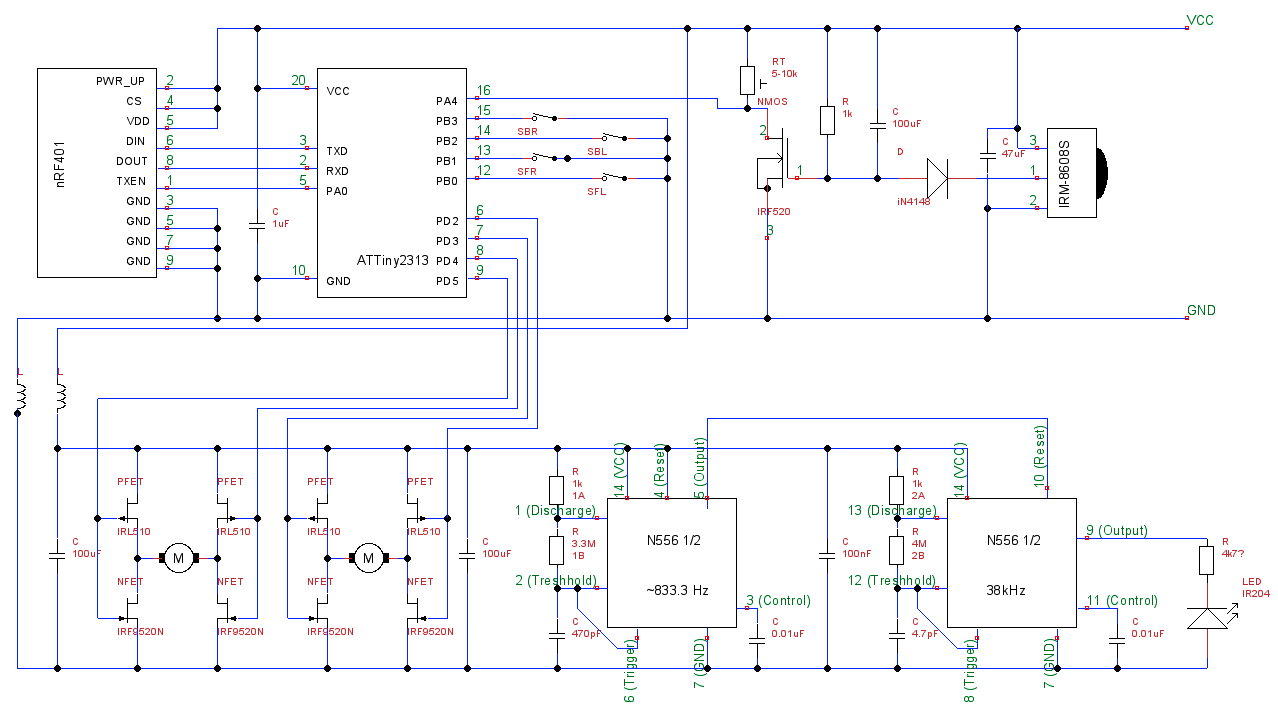
\includegraphics[angle=90,height=0.8\textheight]{tCad1.pdf}
\end{figure}

\begin{figure}[hp]
   \caption{Simple flowchart describing the execution of the software}
   \label{fig:flow}
   \vspace{10mm}
   \centering
      \includegraphics[angle=90]{flow.pdf}
\end{figure}

% \clearpage
% \appendix
% \newpage

\end{document}